\chapter{Code}
\label{chap: Code}

\section{相机内参标定实现}
利用MATLAB的“TOOLBOX\_calib”工具包在输入了标定图片之后会自动标定。标定得到的相机参数如图所示:

\begin{center}
    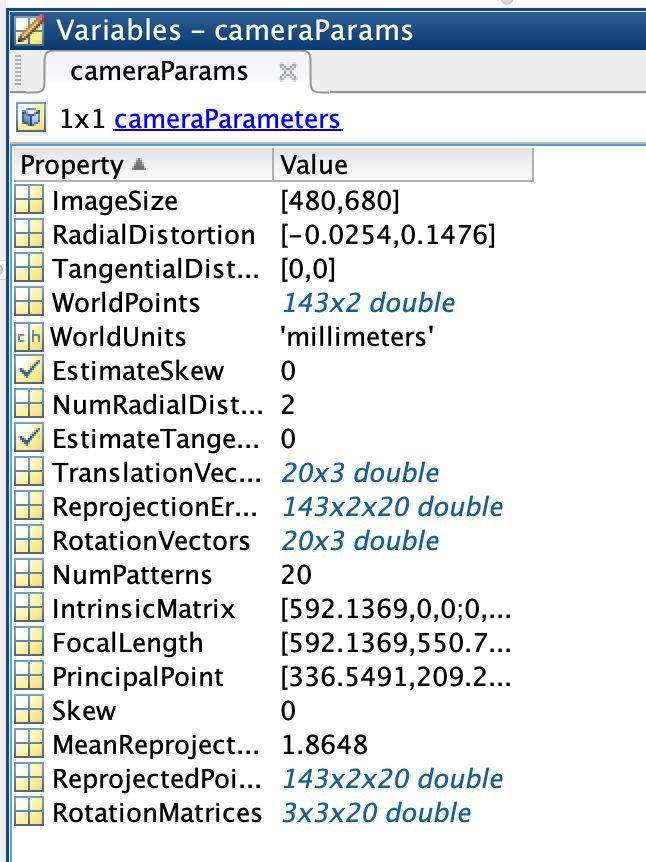
\includegraphics[width=0.4\textwidth]{figures/camera.png}
\end{center}

\section{去畸变}
MATLAB自带去除畸变的函数unditorImage,输入相机内参以及由该相机拍摄的图片即可获得去畸变处理后的图像

\begin{lstlisting}
I1 = undistortImage(I1,mycamera);
I2 = undistortImage(I2,mycamera);
I3 = undistortImage(I3,mycamera);
\end{lstlisting}


\section{特征点匹配}
在实际检测特征点的时候使用了SURF算子,对两张图片首先分别利用detectSURFFeatures函数检测图像的SURF特征点,该函数输入为需要提取特征的图像,返回提取得到的SURF特征点。然后利用extractFeatures函数对上一步提取得到的特征点计算描述向量用于之后的匹配。

extractFeatures函数的输入为图片以及对应的特征点,返回值为SURF描述子(特征描述向量)以及对应该描述子的点的位置。

\begin{lstlisting}
SURF_Pt_1 = detectSURFFeatures(rgb2gray(I1));
SURF_Pt_2 = detectSURFFeatures(rgb2gray(I2));
[features_1,validPoints_1] = 
    extractFeatures(rgb2gray(I1),SURF_Pt_1);
[features_2,validPoints_2] =   
    extractFeatures(rgb2gray(I2),SURF_Pt_2);
\end{lstlisting}

利用描述子做匹配的过程主要运用了matchFeatures函数,该函数输入为两个图像的特征描述子,返回的是匹配之后的匹配点的索引,index,其中index为n*2的矩阵,第一列对应第一张图像的匹配点的索引,第二列对应第二张图像的匹配点的索引。有了该索引,结合extractFeatures函数输出的描述向量对应点的位置,即可得到两张图片的匹配点。在匹配的过程中,为了降低outlier的比例,利用最佳匹配和第二好匹配的特征描述子距离比值进行筛选,对应于matchFeatures函数的'Maxratio'参数,在这里按照老师的建议设置为0.7。在得到了匹配点的位置之后就可以进行显示,显示函数为showMatchedFeatures。

\section{使用RANSAC进行基础矩阵的估算}
利用RANSAC进行基础矩阵及本征矩阵的估算的实现,可以调用Computer Vision System Toolbox 工具箱中的estimateFundamentalMatrix和estimateEssentialMatrix函数。
我利用第4步求出的匹配点集,调用estimateFundamentalMatrix函数,该函数的输入为两组相互匹配的点集,以及一些(name,value)对,在这里设置’Method’为‘RANSAC’,即使用RANSAC方法对该匹配进行基础矩阵求解。该函数在返回基础矩阵F的同时还返回了对应于该基础矩阵的内点。在这个迭代过程之后,将返回的内点送入estimateEssentialMatrix函数再计算一遍本征矩阵,由于输入已经是内点,且考虑时间成本,该计算过程不需要RANSAC迭代,可直接得到对于本征矩阵E的较精确的估计。

\begin{lstlisting}
[F, inliers] = estimateFundamentalMatrix(
    matchedPoints1_12,matchedPoints2_12,'Method','RANSAC');
inlierPoints1_12 = 
    matchedPoints1_12(inliers,:);
inlierPoints2_12 = 
    matchedPoints2_12(inliers,:);
figure;
showMatchedFeatures(I1, I2, inlierPoints1_12,
    inlierPoints2_12,'montage','PlotOptions',{'ro','go','y--'});
title('Point matches after outliers were removed');
%重新把inliner拿去重新算一遍Fundamental Matrix
[F,inliers] = estimateFundamentalMatrix(
    inlierPoints1_12, inlierPoints2_12, 'Method', 'RANSAC');
\end{lstlisting}

\section{从基础矩阵中分解旋转矩阵与平移矩阵}
显然在通过两个图像点的匹配求得对应的本征矩阵之后,可直接由本征矩阵结合相机参数估算两个视角的相对旋转矩阵与平移矩阵。该过程可利用MATLAB中的relativeCameraPose函数和cameraPoseToExtrinsics函数。其中relativeCameraPose函数输入为本征矩阵、相机内参以及对应的匹配内点。该函数的作用即将联系两张图像的本征矩阵转化成对应的相机相对位置。返回的参数即相对方向和相对距离。将这两个返回参数送入cameraPoseToExtrinsics函数就可以将该相对方向和距离转化为相对旋转矩阵和平移矩阵。对于第一张图像的相机位姿而言,它在这个过程中是起到参照物的作用,因此它的相对方向和距离矩阵分别为单位阵和零矩阵。将单位阵和零矩阵输入cameraPoseToExtrinsics函数便可得到在第一个相机位姿的参照下,其本身的旋转矩阵和平移矩阵。

\begin{lstlisting}[language=matlab]
Ori1 = [1,0,0; 0,1,0; 0,0,1];
Loc1 = [0,0,0];
[M_rot1, M_trans1] = cameraPoseToExtrinsics(Ori1, Loc1);

[reOri_12, reLoc_12] = relativeCameraPose(
    F, mycamera, inlierPoints1_12, inlierPoints2_12);
[M_rot2, M_trans2] = 
    cameraPoseToExtrinsics(reOri_12, reLoc_12);
\end{lstlisting}

\section{三角化三维点云重构}
当我们知道两张图像的对应匹配点,同时还得到了两个成像相机的相机矩阵,就可以用三角法重构出这些点在三维坐标下的位置。在MATLAB实现的过程中,调用了cameraMatrix函数,输入相机参数以及对应的相机的旋转矩阵和平移矩阵,返回该相机矩阵。对两个相机位姿拍下的图分别调用该函数,即可得到两个相机矩阵,将相机矩阵与两张图中的匹配点输入triangulate函数进行三角化,即可得到在三维坐标系下各点的位置

\begin{lstlisting}
Cam1 = cameraMatrix(cameraParams, eye(3), [0 0 0]);
Cam2 = cameraMatrix(mycamera,M_rot2,M_trans2);
worldPoint = triangulate(
    matchedPoints1_12,matchedPoints2_12,Cam1,Cam2);
\end{lstlisting}

\section{得到第三张图的3D-2D对应关系}
我已经得到了在第一个相机参照下的三维点云,我们再对第一张图片与第三张进行SURF特征匹配,并根据匹配点在三维坐标系下的坐标得到对应第三个相机的部分点在三维坐标系下的坐标,由于我们的三维坐标系是以第一个相机为中心建立的,因此由这些点在三维坐标系下的位置我们又可以估算第三个相机相对第一个相机的位姿。

\begin{lstlisting}
SURF_Pt_3 = detectSURFFeatures(rgb2gray(I3));
[features_3,validPoints_3] = 
    extractFeatures(rgb2gray(I3),SURF_Pt_3);
indexPairs2 = matchFeatures(features_1, 
    features_3, 'MaxRatio', 0.7, 'Unique', true);
matchedPoints1_13 = validPoints_1(indexPairs2(:,1));
matchedPoints3_13 = validPoints_3(indexPairs2(:,2));
[asd,index12_1,index13_1] = 
    intersect(indexPairs(:,1),indexPairs2(:,1));
worldPoint_i3 = worldPoint(index12_1,:);
pixelPoint_i3 = 
    matchedPoints3_13(index13_1,:).Location;
\end{lstlisting}


\section{使用RANSAC方法估算第三个视角位置}
我们已经知道了第三张图片的点在三维空间中的坐标,我们就可以利用MATLAB的estimateWorldCameraPose函数估算出在三维空间里的相机3的方向与距离矢量。由于我们的三维空间是以第一个相机的位姿为中心建立的,因此这个位姿就是相机3相对相机1的位姿(对应P3P算法)。在MATLAB实现过程中首先用estimateWorldCameraPose函数估算相机3在三维空间里的方向和距离,再利用cameraPoseToExtrinsics函数得到该方向和距离对应的旋转矩阵和平移矩阵。

\begin{lstlisting}
[reOri_13, reLoc_13] = estimateWorldCameraPose(
    pixelPoint_i3,worldPoint_i3,mycamera);
[M_rot3, M_trans3] = 
    cameraPoseToExtrinsics(reOri_13, reLoc_13);
Cam3 = cameraMatrix(mycamera,M_rot3,M_trans3);
\end{lstlisting}
    

\section{Bundle Adjustment}
在matlab中调用Bundle Adjustment函数需要4个参数,分别是xyzPoints,pointTracks,cameraPoses,cameraParams,即世界坐标系中的点,在相机上的投影点,相机的姿态,相机的参数。

为了生成pointTracks,我调用的matlab自带的viewSet函数来生成各个相机的信息序列。

\begin{lstlisting}
vSet = viewSet;
vSet = addView(vSet, 1,'Points',validPoints_1,'Orientation',...
    M_rot1,'Location',M_trans1);
vSet = addView(vSet, 2,'Points',validPoints_2,'Orientation',...
    M_rot2,'Location',M_trans2);
vSet = addConnection(vSet,1,2,'Matches',indexPairs);
vSet = addView(vSet, 3,'Points',validPoints_3,'Orientation',...
    M_rot3,'Location',M_trans3);
vSet = addConnection(vSet,1,3,'Matches',indexPairs2);

tracks = findTracks(vSet);
cameraPoses = poses(vSet);
\end{lstlisting}

从而得到了pointTrack以及cameraPoses。
然后就是调用Bundle Adjustment函数,得到refined的点云坐标以及相机姿态
\begin{lstlisting}
[xyzPoints,errors] = triangulateMultiview(...
    tracks,cameraPoses,cameraParams);

[xyzRefinedPoints,refinedPoses] = ...
    bundleAdjustment(xyzPoints,tracks,cameraPoses,cameraParams);
\end{lstlisting}
